


  \documentclass[letterpaper,11pt]{article}
  \usepackage{latexsym}
  \usepackage[empty]{fullpage}
  \usepackage[usenames,dvipsnames]{color}
  \usepackage{verbatim}
  \usepackage{hyperref}
  \usepackage{framed}
  \usepackage{tocloft}
  \usepackage{bibentry}
  \usepackage{amsmath}
  \usepackage{scrextend}
  \usepackage{listings}
  \usepackage{color}
  \usepackage{fancyhdr}
  \usepackage{graphicx}
  \usepackage{pgfplots}

  %THIS PORTION IS FOR ADDING PAGE NUMBER
  \pagestyle{fancy}
  \cfoot{}
  \rfoot{\thepage}
  \renewcommand{\headrulewidth}{0pt}
  %THIS PORTION IS FOR ADDING PAGE NUMBER.


  \urlstyle{same}
  \definecolor{mygrey}{gray}{.85}
  \definecolor{mygreylink}{gray}{.30}
  \textheight=9.0in
  \raggedbottom
  \raggedright
  \setlength{\tabcolsep}{0in}


  %The following part is for inserting codes in LaTeX:
  \definecolor{codegreen}{rgb}{0,0.6,0}
  \definecolor{codegray}{rgb}{0.5,0.5,0.5}
  \definecolor{codepurple}{rgb}{0.58,0,0.82}
  \definecolor{backcolour}{rgb}{0.95,0.95,0.92}

  \lstdefinestyle{mystyle}{
      backgroundcolor=\color{backcolour},
      commentstyle=\color{codegreen},
      keywordstyle=\color{magenta},
      numberstyle=\tiny\color{codegray},
      stringstyle=\color{codepurple},
      basicstyle=\footnotesize,
      breakatwhitespace=false,
      breaklines=true,
      captionpos=b,
      keepspaces=true,
      numbers=left,
      numbersep=5pt,
      showspaces=false,
      showstringspaces=false,
      showtabs=false,
      tabsize=2
  }
  \lstset{style=mystyle}
  %For inserting codes in LaTeX

  \begin{document}

  \begin{center}
  	\textbf{\Huge{Advanced Data Analysis HW1}}
  \end{center}

  \begin{center}
  	\textsl{Ao Liu, al3472}
  \end{center}


  \bigbreak
  \bigbreak
  \bigbreak

  %%%%%%%%%%%%%%%%%%%%%%%%%%%%%%%%%%%%%
  %%%%%%%%%%%%%%   1   %%%%%%%%%%%%%%%%
  %%%%%%%%%%%%%%%%%%%%%%%%%%%%%%%%%%%%%


    \begin{addmargin}[-2em]{0em} \large{\textbf{1. }}\end{addmargin}
    \begin{addmargin}[-1.1em]{0em} \textbf{Let $\eta$ denote the median of a random variable X. Consider testing $H_0: \eta = 0$ against $H_a: \eta \neq 0$ using $X_1,X_2,...,X_{25}$, a random sample of size $n = 25$ from the distribution of $X$}\par \end{addmargin}


  \begin{addmargin}[-1.1em]{0em} \textbf{(a)  Let $S$ denote the sign statistic. Determine the level of the test that rejects $H_0$ if $S\geq16$.}\par \end{addmargin}


    \bigbreak
    \begin{addmargin}[-0.5em]{0em}
    \textbf{Answer: }\end{addmargin}

Let the sign test $S = \sum_{i=1}^{25}I(X_i\geq0)$, then $S\sim Bin(25,\frac{1}{2})$
If under certain level the test will reject $H_0$ if $S\geq16$, then according to symmetry, the test will also reject $H_0$ if $S\leq9$.\par
So the level of the test is:\par
$$p(S\geq16 or S\leq9)=0.2295$$
\bigbreak


\begin{addmargin}[-1.1em]{0em}
\textbf{(b)}\par\end{addmargin}
  \textbf{Determine the power of the teat in
  (a) if $X$ has $N(0.5,1)$ distribution?} \par
\bigbreak

\begin{addmargin}[-0.5em]{0em}
\textbf{Answer: }\end{addmargin}


If $X\sim N(0.5,1)$, then $P(X\geq0)=0.6915$, so $S\sim Bin(25,0.6915)$.
So the power of the test is:
$$1-p(9<S<16\vert H_\alpha)=0.7842$$

%%%%%%%%%%%%%%%%%%%%%%%%%%%%%%%%%%%%%
%%%%%%%%%%%%%%   2   %%%%%%%%%%%%%%%%
%%%%%%%%%%%%%%%%%%%%%%%%%%%%%%%%%%%%%


  \begin{addmargin}[-2em]{0em} \large{\textbf{2. }}\end{addmargin}

  \begin{addmargin}[-1.1em]{0em} \textbf{The data in in the talble below gives the pretest and posttest scores on the MLA listening test in Spanish for 20 high school teachers who attended an intensive course in Spanish.}\par\end{addmargin}
  \bigbreak

  \begin{center}
  \begin{tabular}{ p{2cm}p{2cm}p{2cm}p{2cm}p{2cm}p{2cm}  }
     \\
    \centering subject & pretest & posttest & subject & pretest & posttest\\
   \hline
  \centering 1 &30 &20 &11 &30 &32\\
  \centering 2 &28 &30 &12 &29 &22\\
  \centering 3 &31 &32 &13 &31 &34\\
  \centering 4 &26 &30 &14 &29 &32\\
  \centering 5 &20 &16 &15 &34 &32\\
  \centering 6 &30 &25 &16 &20 &27\\
  \centering 7 &34 &31 &17 &26 &28\\
  \centering 8 &15 &18 &18 &25 &29\\
  \centering 9 &28 &33 &19 &31 &32\\
  \centering 10 &20 &25 &20 &29 &32\\
  \end{tabular}
  \end{center}

  \begin{addmargin}[-1.1em]{0em} \textbf{Assume that the differences between these scores (pretest scores −posttest) constitute a
random sample from a distribution $F$ with mean $mu$ and variance $\sigma^2$}\par\end{addmargin}
  \bigbreak

  \begin{addmargin}[-1.1em]{0em}
  \textbf{(a)}\par\end{addmargin}
    \textbf{Use a t-test and $\alpha = 0.05$ to test $H_0:\mu = 0$ against $H_\alpha: \mu = 0$. What is the p-value of the test? What assumption you need to make. Use a graphical technique to check this assumption.}\par
  \bigbreak
  \begin{addmargin}[-0.5em]{0em}
  \textbf{Answer: }\end{addmargin}


  %insert code snippets:
  \begin{lstlisting}
  pre <- c(30,28,31,26,20,30,34,15,28,20,30,29,31,29,34,20,26,25,31,29)
  post <- c(20,30,32,30,16,25,31,18,33,25,32,22,34,32,32,27,28,29,32,32)
  score <- pre-post
  t.test(score,mu=0)
  \end{lstlisting}

  and we get the following result:

\begin{lstlisting}
One Sample t-test

data:  score
t = -0.7054, df = 19, p-value = 0.4891
alternative hypothesis: true mean is not equal to 0
95 percent confidence interval:
 -2.77699  1.37699
sample estimates:
mean of x
     -0.7
\end{lstlisting}

The p-value of the test is 0.4891\par
In order to make the t-test result more plausible, we have to make an assumption that the underlying dietribution is not extremely skewed. To check our assumption, we make a qq plot of the given data:\par

\begin{lstlisting}
  qqnorm(y)
  qqline(y, col = 1)
\end{lstlisting}


The following is a way to insert pics:
\begin{center}
  \makebox[\linewidth]{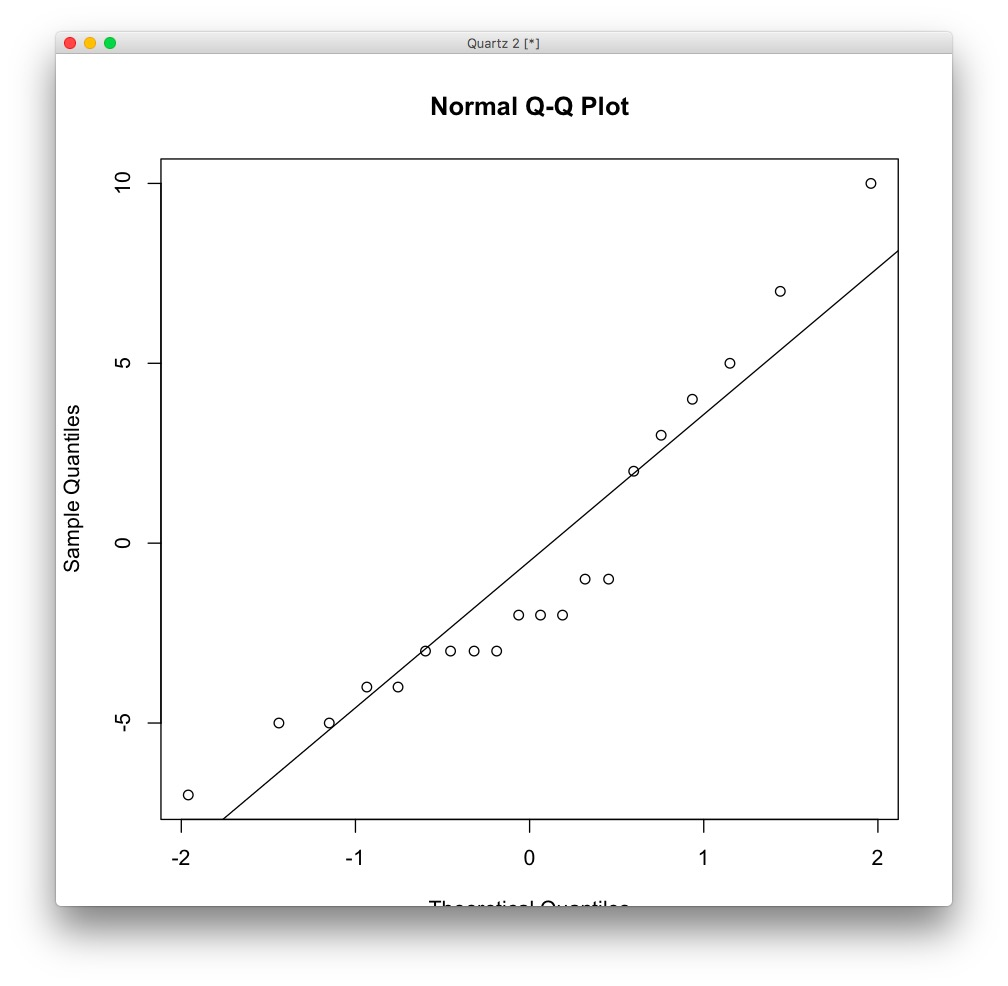
\includegraphics[width=\textwidth]{ADAHW1.jpg}}
\end{center}

As we can see from the figure, our assumption is met.


  \bigbreak
  \begin{addmargin}[-1.1em]{0em}
  \textbf{(b)}\par\end{addmargin}
    \textbf{Obtain a $95\%$ confidence interval for the mean in (a) }\par
  \bigbreak
  \begin{addmargin}[-0.5em]{0em}
  \textbf{Answer: }\end{addmargin}

From the result that we get from (a), the $95\%$ confidence interval is:
$$(-2.77699, 1.37699)$$

  \bigbreak
  \begin{addmargin}[-1.1em]{0em}
  \textbf{(c)}\par\end{addmargin}
    \textbf{If the median of $F$ is $\eta$,use the sign test and $\alpha$=0.05 to test $H_0: \eta=0$ against $H_\alpha: \eta\neq 0$. What is the p-value of this test?}\par
  \bigbreak
  \begin{addmargin}[-0.5em]{0em}
  \textbf{Answer: }\end{addmargin}
The values of "score" are:
\begin{lstlisting}
[1] 10 -2 -1 -4  4  5  3 -3 -5 -5 -2  7 -3 -3  2 -7 -2 -4 -1 -3
\end{lstlisting}
It turns out there are 6 positive socres in the sample. \par
So we do the following sign test:

  \begin{lstlisting}
    Exact binomial test

    data:  6 and 20
    number of successes = 6, number of trials = 20, p-value = 0.1153
    alternative hypothesis: true probability of success is not equal to 0.5
    95 percent confidence interval:
     0.1189316 0.5427892
    sample estimates:
    probability of success
                       0.3

  \end{lstlisting}
The p-value of this test is 0.1153

  \bigbreak
  \begin{addmargin}[-1.1em]{0em}
  \textbf{(d)}\par\end{addmargin}
    \textbf{Obtain a $95\%$ confidence interval for $\eta$ and compare use answer the answer in (b)}\par
  \bigbreak
  \begin{addmargin}[-0.5em]{0em}
  \textbf{Answer: }\end{addmargin}

According to the result in (c), the $95\%$ confidence interval for $\eta$ is:
$$(0.1189316, 0.5427892)$$

Compared with the confidence interval that we get in the t test above, this one is smaller, more accurate.

  %%%%%%%%%%%%%%%%%%%%%%%%%%%%%%%%%%%%%
  %%%%%%%%%%%%%%   3   %%%%%%%%%%%%%%%%
  %%%%%%%%%%%%%%%%%%%%%%%%%%%%%%%%%%%%%

  \bigbreak
  \begin{addmargin}[-2em]{0em} \large{\textbf{3. }}\end{addmargin}

  \begin{addmargin}[-1.1em]{0em} \textbf{Twelve one week old infants were randomly assigned into two groups of six infant each. One group participated in an experimental active-exercise to learn to walk and the other was used as a control group. The following are the ages at which these infants first walked alone}\par\end{addmargin}

  \bigbreak
  \begin{center}
  \begin{tabular}{ p{6cm}p{6cm} }
     \\
    \centering Active-exercise group & No-exercise group\\
   \hline
  \centering 9.00 &11.50\\
  \centering 9.50 &12.00\\
  \centering 9.75 &9.00\\
  \centering 10.00 &11.50\\
  \centering 13.00 &13.25\\
  \centering 9.50 &13.00\\

  \end{tabular}
  \end{center}

Call the no-exercise group Y sample and the active-exercise group X sample. Compare the two groups using two tests (one parametric and one nonparametric) (take α = 0.05). State all the assumptions that you make in carrying out these tests.

\bigbreak

  \textbf{Answer: }\end{addmargin}
  \bigbreak


  (1) Non Parametric Test:\par
  (Wilcoxon) Mann-Whitney two sample procedure:\par
  We assume that the populations have the same shape and differ only in location.


\begin{lstlisting}
  active <- c(9.00,9.50,9.75,10.00,13.00,9.50)
  no <- c(11.50,12,9,11.50,13.25,13)
  wilcox.test(active,no,correct = FALSE)
\end{lstlisting}

\begin{lstlisting}
  Wilcoxon rank sum test with continuity correction

data:  active and no
W = 9, p-value = 0.1705
alternative hypothesis: true location shift is not equal to 0

Warning message:
In wilcox.test.default(active, no) : cannot compute exact p-value with ties
\end{lstlisting}
\bigbreak

Since p-value is 0.1705, we cannot reject the Null Hypothesis.
\bigbreak

(2) Parametric Test:
We use ANOVA F-Test to check whether the two population have the same mean.\par
Assume every population of interest has unknown population mean and variance.

\begin{lstlisting}
level <- c(rep("active", 6), rep("no", 6))
age <- c(9, 9.5, 9.75, 10, 13, 9.5, 11.5, 12, 9, 11.5, 13.25, 13)
data <- data.frame(level, age)
summary(aov(age ~ level))
\end{lstlisting}
%http://www.r-tutor.com/elementary-statistics/non-parametric-methods/mann-whitney-wilcoxon-test

\begin{lstlisting}
Df Sum Sq Mean Sq F value Pr(>F)
level        1  7.521   7.521   3.415 0.0943 .
Residuals   10 22.021   2.202
---
Signif. codes:  0 ‘***’ 0.001 ‘**’ 0.01 ‘*’ 0.05 ‘.’ 0.1 ‘ ’ 1
[Finished in 0.497s]
\end{lstlisting}

So $SSB = 7.521$, $SSE = 22.021$,
$MSB = 7.521$, $MSE = 2.2021$, $F=3.415$

If we take $\alpha = 0.05$, we have


\begin{lstlisting}
>qf(.95, df1=1, df2=10)
[1] 4.964603
\end{lstlisting}

$F(1-0.05,1,10) = 4.965$

Since $3.415>4.965$, we cannot reject $H_0$
\bigbreak
Also, p-value = $0.0943>0.05$, we cannot reject $H_0$


\end{document}
%Insert pics:
%%%%%%%%%%%%%
%\begin{center}
  %\makebox[\linewidth]{\includegraphics[width=\textwidth]{4640HW6.jpg}}
%\end{center}



%insert a complicated tab...
%%%%%%%%%%%%%%%%%%%%%%%%%%%%
%\begin{center}
%\begin{tabular}{ p{12cm}p{1cm}p{1cm}p{1cm}  }
%& \multicolumn{3}{c}{Posterior Quantiles} \\
%\centering{Quantity of Interest} & 25\% & 50\% & 75\% \\
%\hline
%geometric mean for Blue Earth (no basement), exp($\beta_2)$ &4.1& 5.0& 6.5\\
%geometric mean for Blue Earth County (basement), exp($\beta_1+\beta_2)$ &6.1 &7.1 &8.2\\
%geometric mean for Clay County (no basement), exp($\beta_3)$& 3.8& 4.7 &5.8\\
%geometric mean for Clay County (basement), exp($\beta_1+\beta_3)$ &5.6& 6.5& 7.6\\
%geometric mean for Goodhue County (no basement), exp($\beta_4)$ & 3.9 &4.9& 6.2\\
%geometric mean for Goodhue County (basement), exp($\beta_1+\beta_4)$ &5.8& 6.8& 7.9\\
%factor for basement vs. no basement, exp($\beta_1$)&1.1& 1.4 &1.7\\
%geometric sd of predictions, exp($\sigma$)&2.1 &2.2& 2.4\\
%\end{tabular}
%\end{center}



%%%insert code snippets:
%%%%%%%%%%%%%%%%%%%%%%%%
%\begin{lstlisting}
%INSERT CODE HERE
%\end{lstlisting}

%Insert equations with alignment:
%%%%%%%%%%%%%%%%%%%%%%%%%%%%%%%%
